\section{Assignment 2}
Throughout this assignment we will use image A (\autoref{A}) and image B (\autoref{B}) to measure similarity. Both image have been downsampled and then blurred with a Gaussian kernel with sigma being 1. For the three similarity graphs, the results have been normalized such that all optima touch 1.0.
\begin{figure}[h]
	\centering
	\begin{subfigure}{0.4\linewidth}
		\centering
		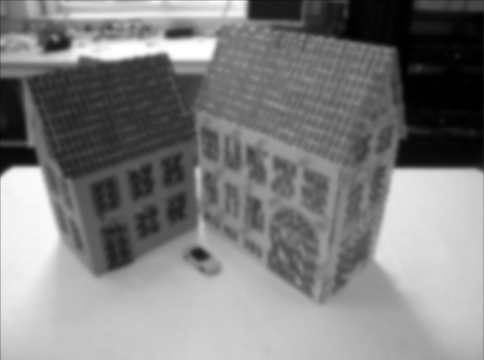
\includegraphics[width=\linewidth]{Materials/A}
		\caption{Image A.}
		\label{A}
	\end{subfigure}
	\hspace{1cm}
	\begin{subfigure}{0.4\linewidth}
		\centering
		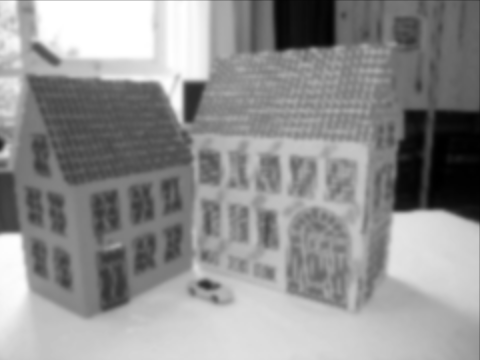
\includegraphics[width=\linewidth]{Materials/B}
		\caption{Image B.}
		\label{B}
	\end{subfigure}
	\caption{}
\end{figure}

\subsection{Self similarity}
We begin our examination of the four similarity measures by looking at self similarity. Here image A is compared to itself. The results can be seen in \autoref{self}.

\begin{figure}[h]
	\centering
	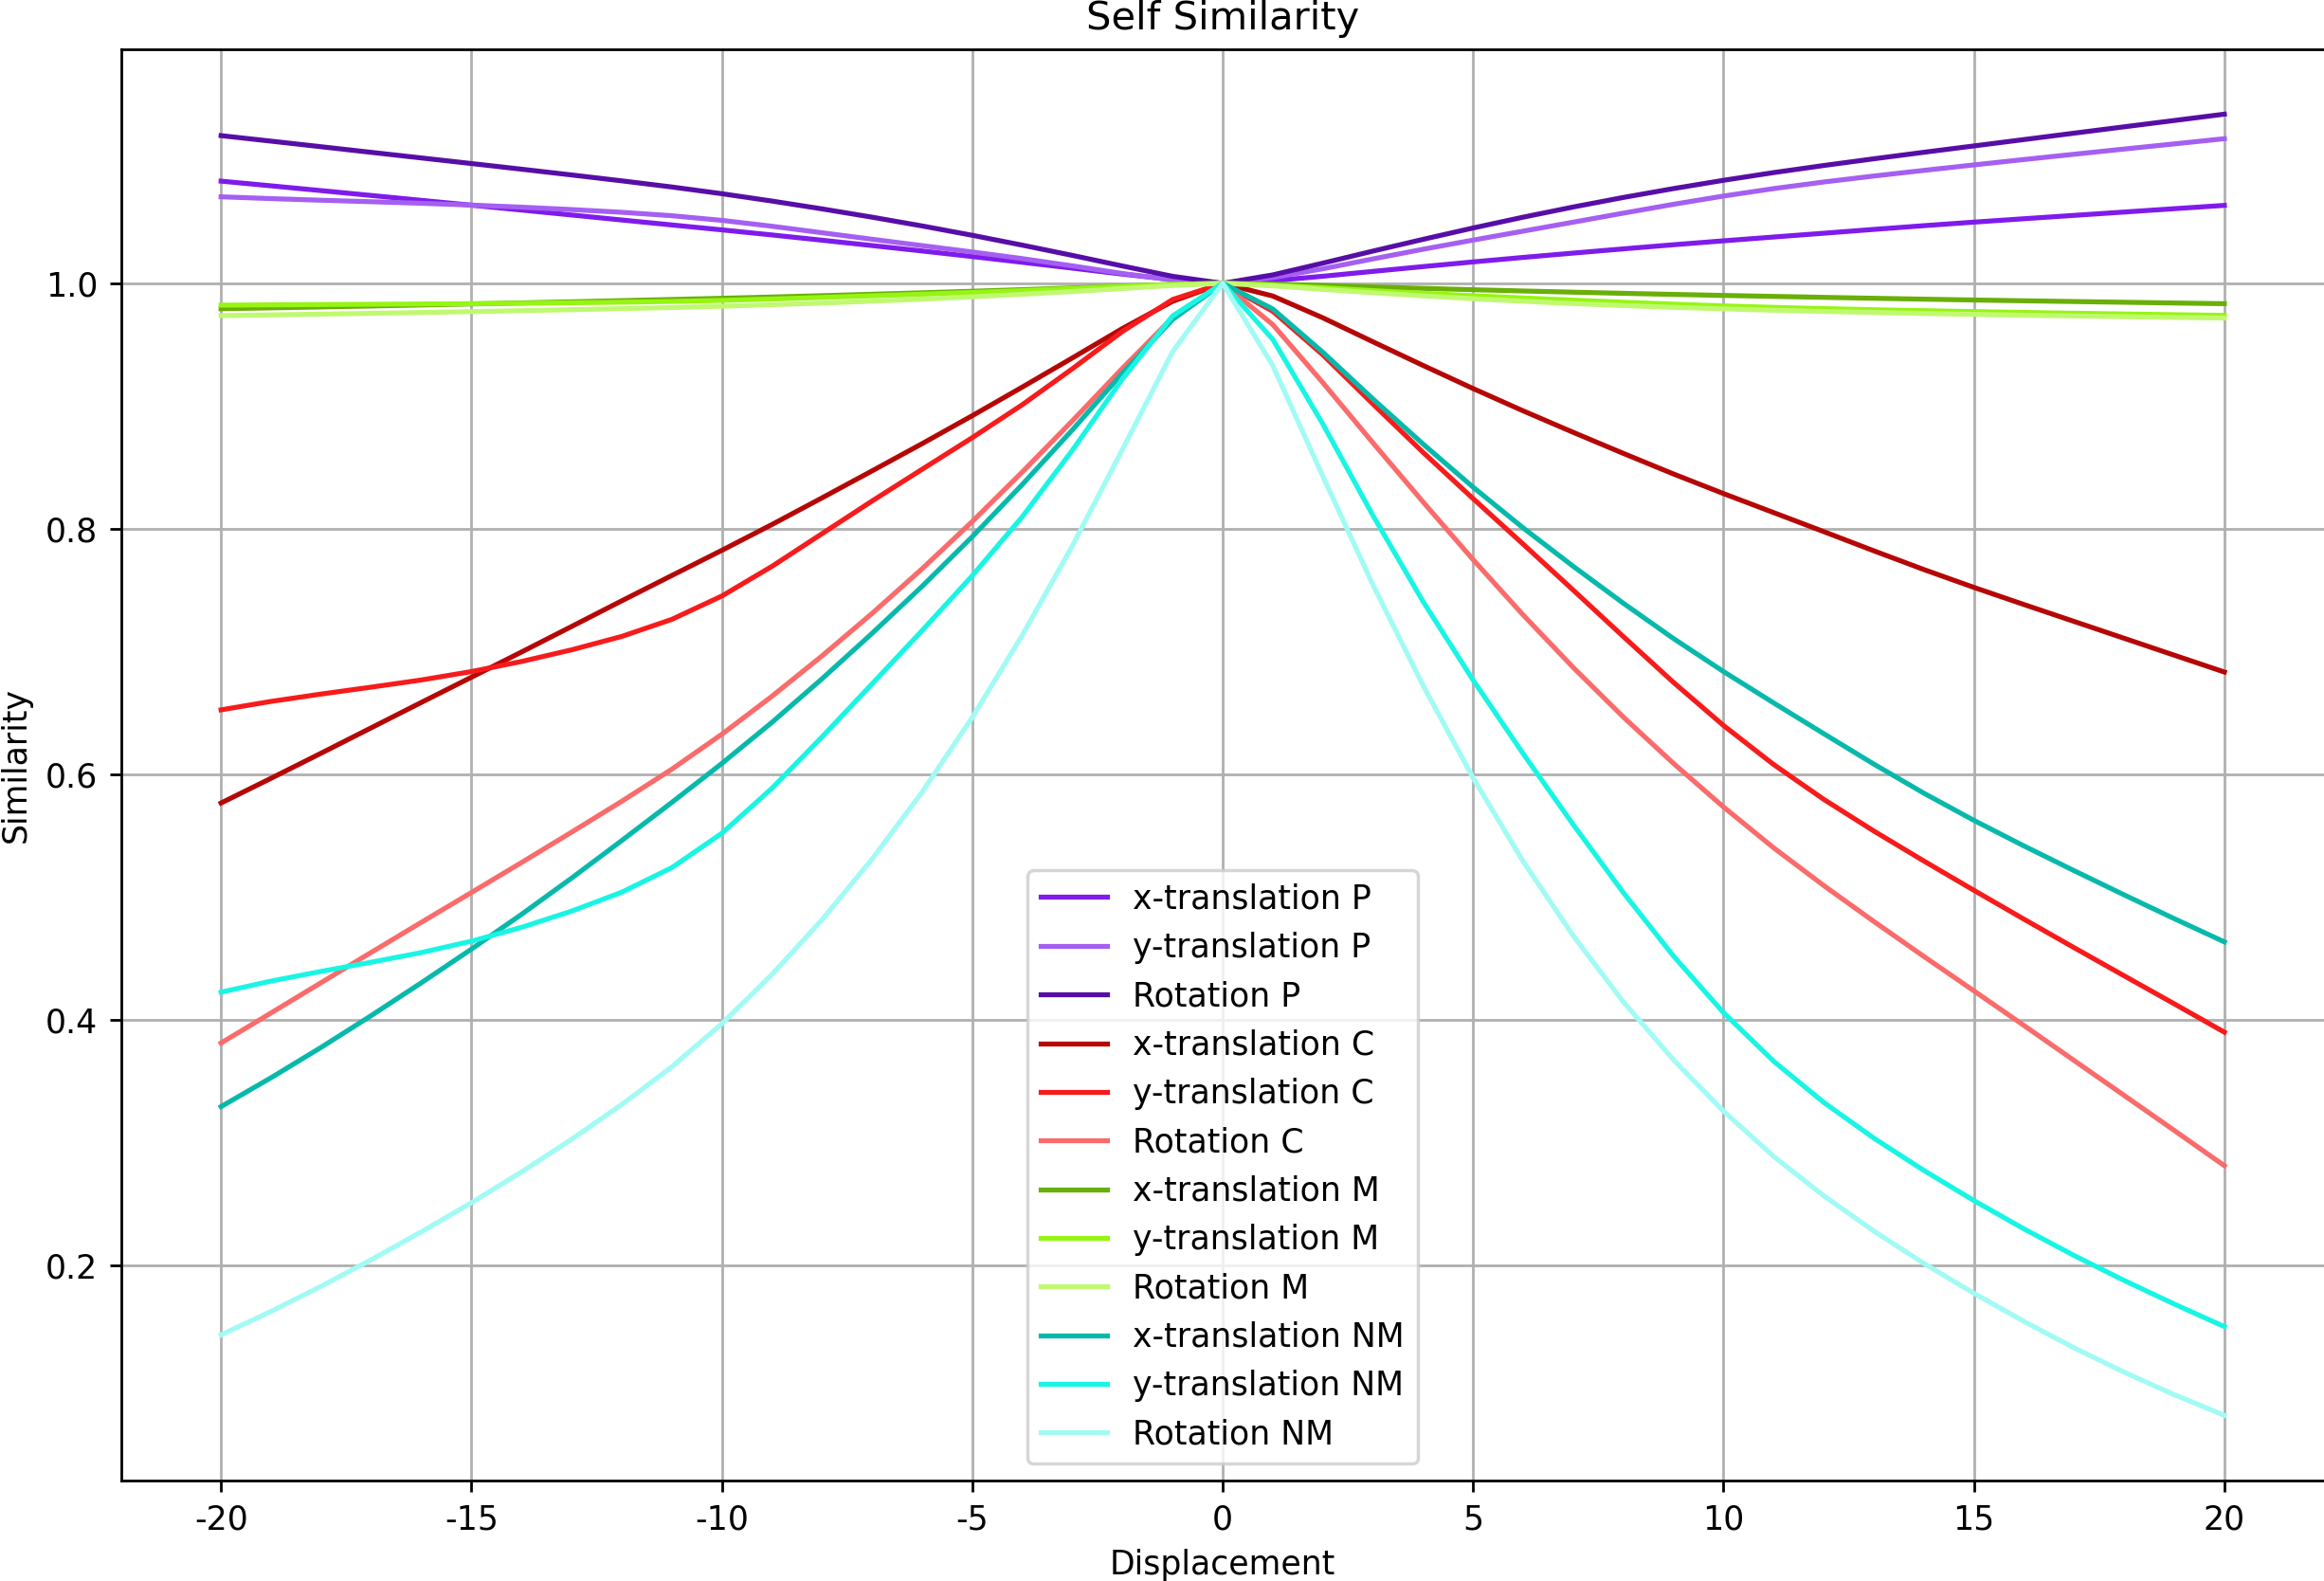
\includegraphics[width=0.8\linewidth]{Materials/selfSimilarity}
	\caption{Self similarity results normalized such that all optima touch 1.0. Both images have been blurred by a Gaussian kernel with sigma being 1. Translation displacement is measured in pixels and rotation displacement is measured in degrees. P = P-norm with P being 2, C = normalized cross correlation, M = mutual information, NM = normalized mutual information.}
	\label{self}
\end{figure}
From the results we note that all similarity measures should be maximized with the exception of P-norm, and thus the P-norm goes above 1.0. We can also see that the similarity measure with the biggest relative difference is NMI, which means NMI both have the greatest gradients, but also is the most sensitive to displacements. In comparison, we see that MI is almost completely flat. However, because MI is so flat, it makes the curves more smooth when we get close to 1.0, whereas for NMI we get some uneven sudden changes as we approach 1.0. For all similarity measures we see them 'peak' at 1.0 as expected as the images should be most similar when not displaced. 
\subsection{Multi modal similarity}
We now take a look at multimodal similarity. Here we have used image A and image A inverted, that is, the intensities have been multiplied by -1. The results can be seen in \autoref{multiModal}.

\begin{figure}
	\centering
	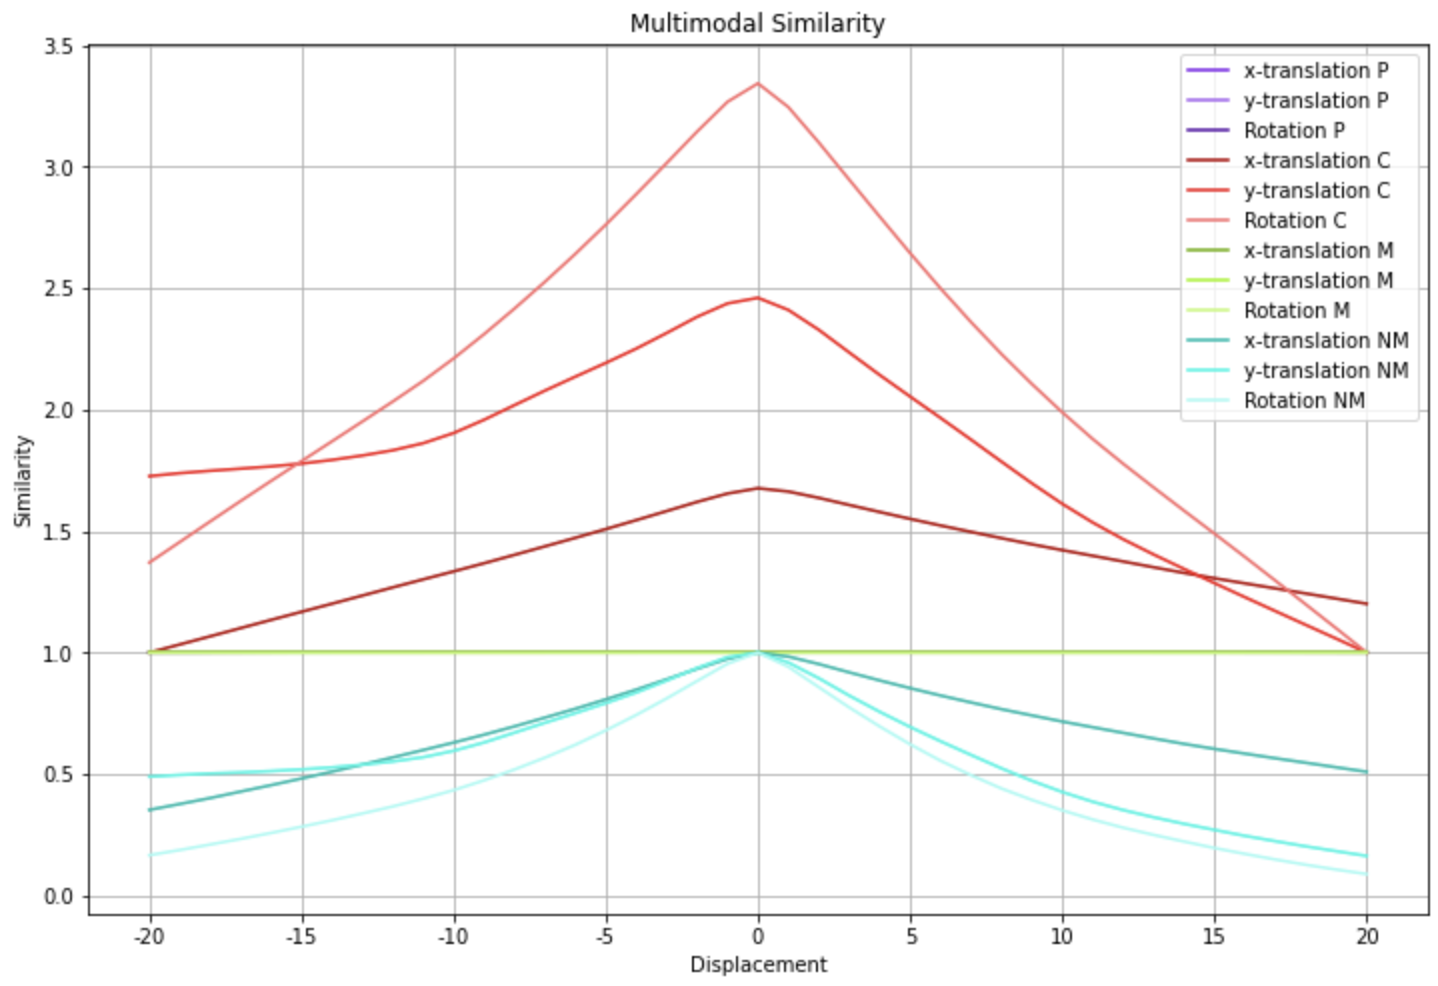
\includegraphics[width=0.8\linewidth]{Materials/multiModalSimilarity}
	\caption{Multi modal similarity results normalized such that all optima touch 1.0. Both images have been blurred by a Gaussian kernel with sigma being 1. Translation displacement is measured in pixels and rotation displacement is measured in degrees. P = P-norm with P being 2, C = normalized cross correlation, M = mutual information, NM = normalized mutual information.}
	\label{multiModal}
\end{figure}
Although it is hard to see, we have that the P-norm is slightly above 1.0 except when the displacements are greatest where it touches 1.0, and we have MI is slightly below 1.0 except when we have 0 displacement where it touches 1.0. We note that NCC now finds the optimal similarities when the displacements are greatest and the smallest similarity when the displacements are 0 as we have normalized the similarities such that the optima touches 1.0. This means NCC is not invariant to intensity changes, and thus is not suitable as a similarity measure for multi modal images. The same is the case for P-norm which also has its optima where the displacement is greatest. We see that  MI behaves correctly and thus is invariant to intensity changes, however, MI become extremely flat, and so its gradients are almost 0. This would make it very hard to optimize the similarity measure with a gradient based method, but it is smooth. Lastly we have NMI which also shows invariance to intensity changes and, of the correctly behaving similarity measures, shows the greatest sensitivity to the displacements. This makes the gradients bigger and thus the function easier to optimize. We also see the curves being more smooth than during self similarity.\\
The reason for P-norm and NCC not being invariant to these intensity changes is they both rely on intensities to compute the similarity, and thus, when we invert one of the images we get negative values as part of the similarity measures, which seemingly flips everything around the x-axis. As MI and NMI works on the distribution of the intensities, and not the intensities themselves, it does not matter if the values have been inverted, it only matter whether we observe as many inverted values as non-inverted values, i.e. that the distribution of pixels are the same in the two images.
\subsection{Object similarity}
We now look at the similarity between image A and B. The results can be seen in \autoref{object}.

\begin{figure}
	\centering
	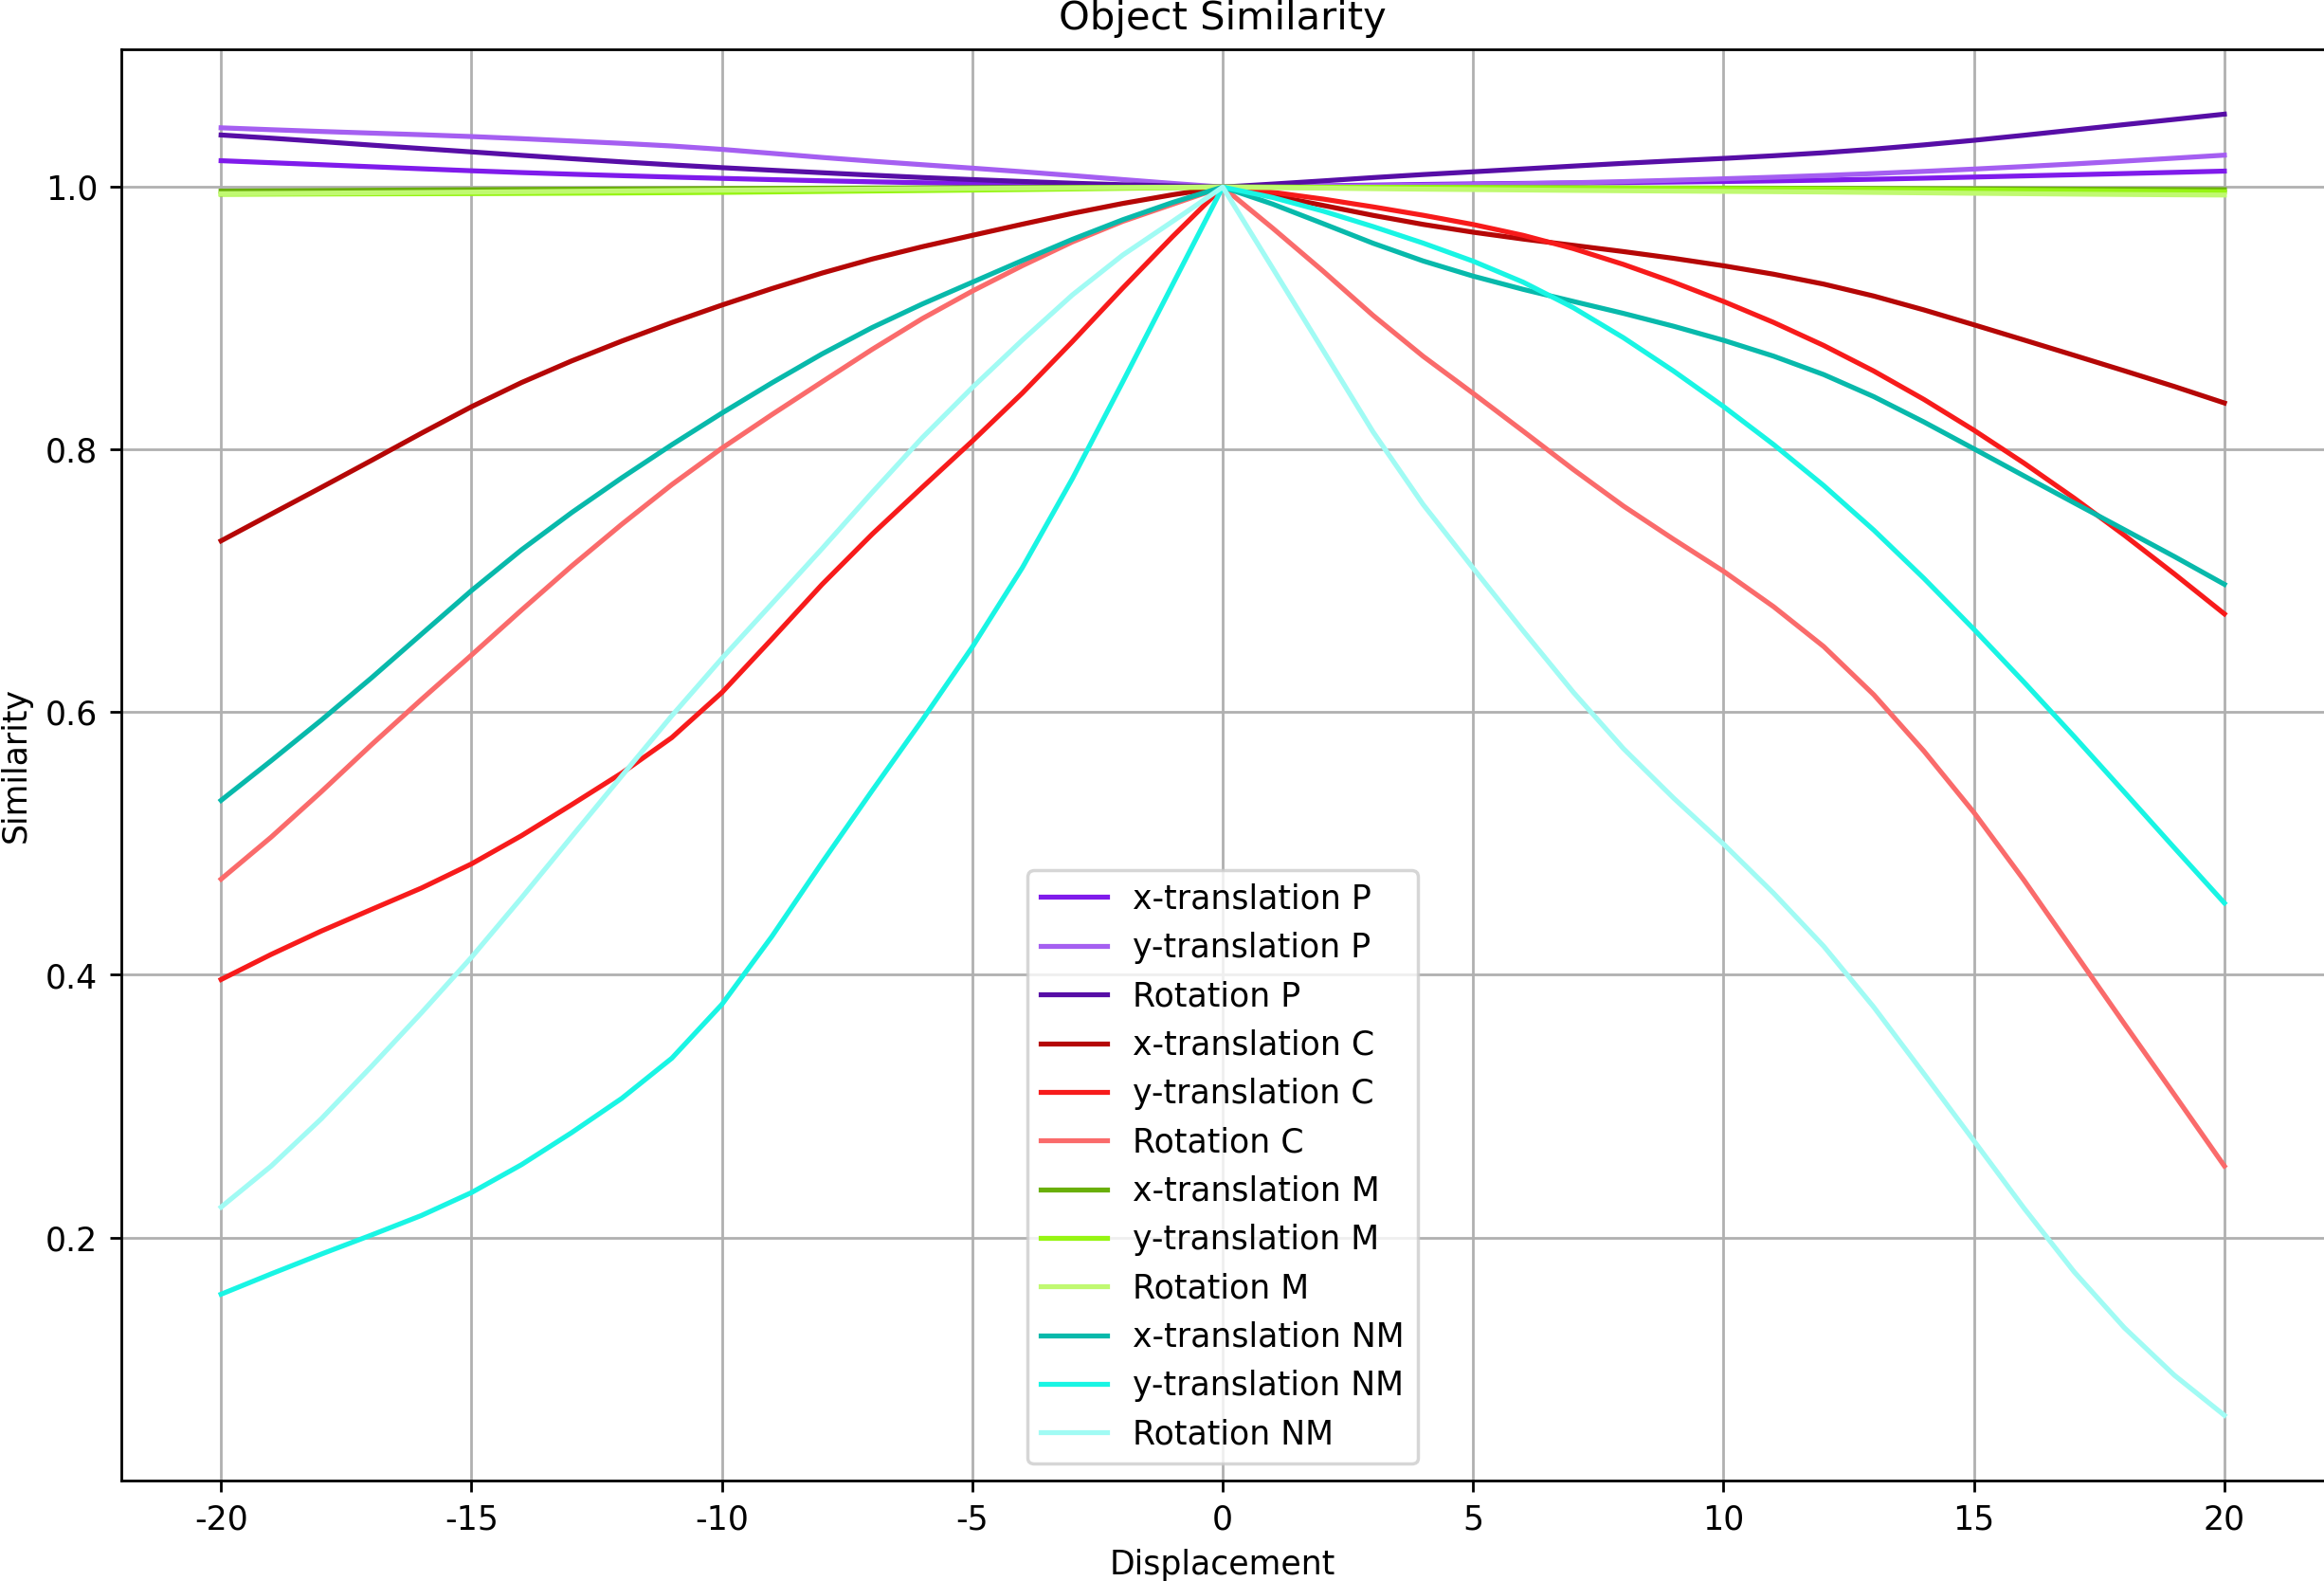
\includegraphics[width=0.8\linewidth]{Materials/objectSimilarity}
	\caption{Object similarity results normalized such that all optima touch 1.0. Both images have been blurred by a Gaussian kernel with sigma being 1. Translation displacement is measured in pixels and rotation displacement is measured in degrees. P = P-norm with P being 2, C = normalized cross correlation, M = mutual information, NM = normalized mutual information.}
	\label{object}
\end{figure}
We here see that all similarity measures again behaves correctly, however, compared to the self similarity results in \autopageref{self} the graphs have become more 'pointy' which would indicate the images are less similar as we need a smaller displacement to make the images dissimilar. By looking at the un-normalized similarity values it can also be reported that the similarity at optima has dropped for all similarity measure. However, we still see the optima being at 0 displacement. This might be due to the foreground and background being the most 'dominant' features in the images, and thus translating and rotating these out of the images might result in a bigger dissimilarity than aligning the images on the motif. We also see for NCC and NMI that the curves have become rather uneven / wavy and not as smooth as for self similarity. This is especially true around 1.0. The more wavy shapes of the curves could be an issue if we would like to optimize the functions with a gradient based method as the waves could form local minima and maxima. We see that the gradients of P-norm and MI is even more flat than for self similarity, making them hard to optimize. 
\subsection{Registration}
We can now look at how our similarity measures perform when we make a rigid and affine registration. In the simplest case we can make a rigid self registration (image A with image A) using NMI. Because we know an optimal transformation matrix will have $\theta = 0$, $t_x = 0$ and $t_y = 0$ we can initialize the transformation matrix to have $\theta = 0.2$, $t_x = 5$ and $t_y = 5$ and see if it returns to all zeros. If we let our gradient descend optimizer run for 200 iterations with a rotation learning rate of 1 and a translation learning rate of 100 we get that the final transformation matrix have $\theta =  0.0023$, $t_x = -0.039$ and $t_y = -0.014$ which is very close to our expectation.\\
We can now perform a rigid transformation using NMI again, but this time using image A and B. We begin by initializing $\theta = 0.3$, $t_x = 5$ and $t_y = 5$. The results can be seen in \autoref{rigidNMIAB}.

\begin{figure}[h]
	\centering
	\begin{subfigure}{0.4\linewidth}
		\centering
		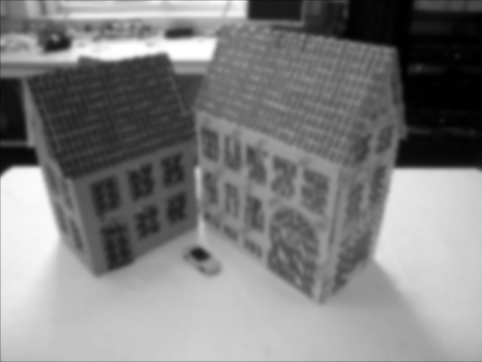
\includegraphics[width=\linewidth]{Materials/rigidNMIAB}
		\caption{Transformed image.\newline}
	\end{subfigure}
	\hspace{1cm}
	\begin{subfigure}{0.4\linewidth}
		\centering
		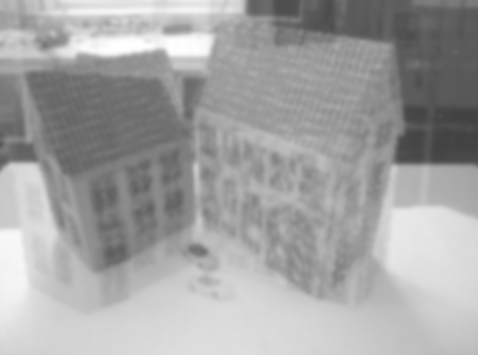
\includegraphics[width=\linewidth]{Materials/rigidNMIABO}
		\caption{Target image overlaid with transformed image.}
	\end{subfigure}
	\caption{Result of rigid registration using NMI on image A and B.}
	\label{rigidNMIAB}
\end{figure}
\begin{figure}
	\centering
	\begin{subfigure}{0.4\linewidth}
		\centering
		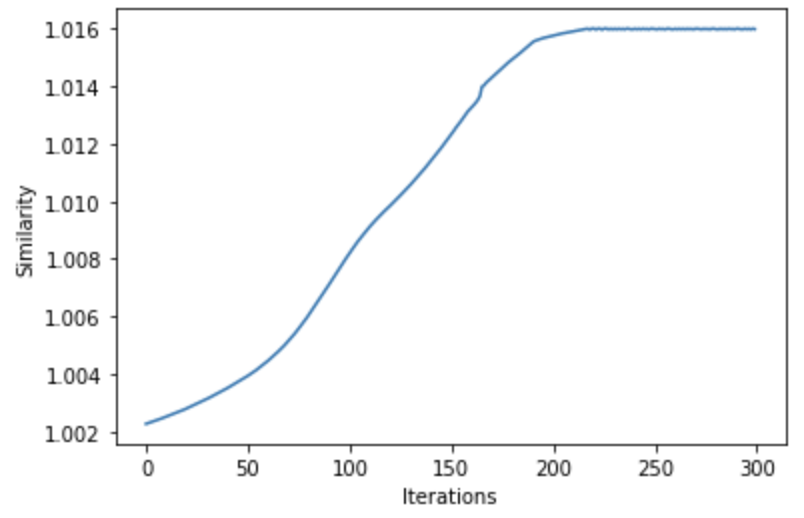
\includegraphics[width=\linewidth]{Materials/RigidNMILoss}
		\caption{Similarity using NMI at each iteration of optimization with translation learning rate of 100 and rotation learning rate at 1.}
		\label{rigidNMIABLoss}
	\end{subfigure}
	\hspace{1cm}
	\begin{subfigure}{0.4\linewidth}
		\centering
		\includegraphics[width=\linewidth]{Materials/RigidNCCLoss}
		\caption{Similarity using NCC at each iteration of optimization with translation learning rate of 10 and rotation learning rate at 0.1.}
		\label{rigidNCCABLoss}
	\end{subfigure}

\end{figure}
We see that the optimized transformation matrix goes towards 0 for all parameters which means it finds the optimal transformation to be no transformation. This is also consistent with the results seen in the object similarity section. In \autoref{rigidNMIABLoss} we see the similarity at each iteration of the optimization, and we see we have found an optima. As discussed earlier, the reason for the optimal parameters being 0 are probably because the foreground is dominant in the images, and optimizing the amount of foreground is probably better than optimizing the overlap of buildings.\\
We can now perform a rigid registration using NCC, image A and image B inverted. Here we initialize with the same parameters, but use a rotation learning rate of 0.1 and a translation learning rate of 10. The results can be seen in \autoref{rigidNCCAB}, and the similarity at each iteration can be seen in \autoref{rigidNCCABLoss}.

\begin{figure}[h]
	\centering
	\begin{subfigure}{0.4\linewidth}
		\centering
		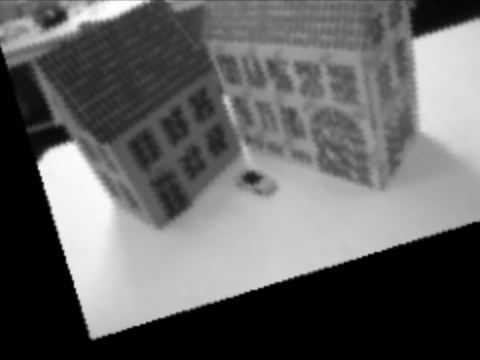
\includegraphics[width=\linewidth]{Materials/rigidNCCAB}
		\caption{Transformed image.\newline}
	\end{subfigure}
	\hspace{1cm}
	\begin{subfigure}{0.4\linewidth}
		\centering
		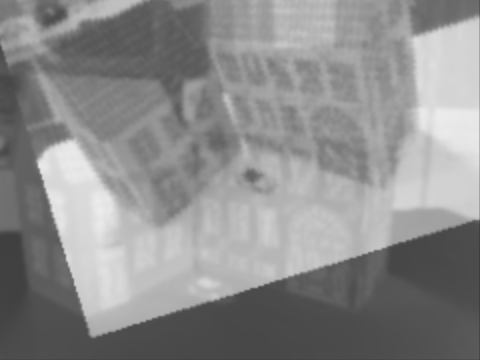
\includegraphics[width=\linewidth]{Materials/rigidNCCABO}
		\caption{Target image overlaid with transformed image.}
	\end{subfigure}
	\caption{Result of rigid registration using NCC on image A and inverted B.}
	\label{rigidNCCAB}
\end{figure}
We here note the motif is getting turned out of the resulting image. This is likely again because the foreground is attempted matched, and rotating the image introduces black pixels into the foreground. This illustrates that NCC is \textit{not} intensity invariant. We also note from \autoref{rigidNCCABLoss} that we have not yet reached an optima, which means if we ran more iterations or used bigger learning rates, the image would get further rotate.\\
We can now perform an affine registration using NMI and image A and B. We initialize the transformation matrix with the same $\theta$, $t_x$ and $t_y$ values as before and initialize $s_x = s_y = 1.2$. The rotation learning rate is set to 0.7, for translation it set to 100, and for scaling it is set to 1. The results can be seen in \autoref{affineNMIAB} and the similarity at each iteration can be seen in \autoref{affineNMIABLoss}.

\begin{figure}[h]
	\centering
	\begin{subfigure}{0.4\linewidth}
		\centering
		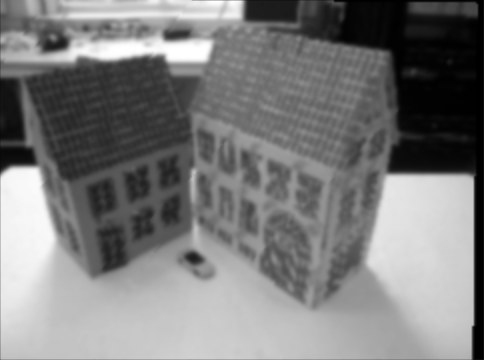
\includegraphics[width=\linewidth]{Materials/affineNMIAB}
		\caption{Transformed image.\newline}
	\end{subfigure}
	\hspace{1cm}
	\begin{subfigure}{0.4\linewidth}
		\centering
		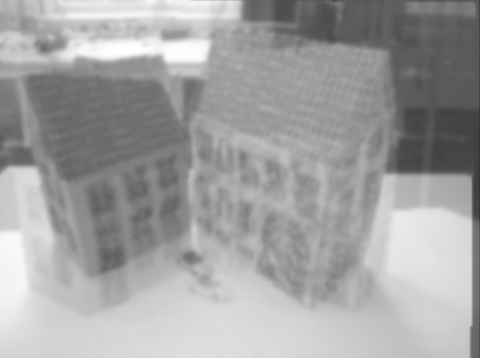
\includegraphics[width=\linewidth]{Materials/affineNMIABO}
		\caption{Target image overlaid with transformed image.}
	\end{subfigure}
	\caption{Result of affine registration using NMI on image A and B.}
	\label{affineNMIAB}
\end{figure}
\begin{figure}[h]
	\centering
	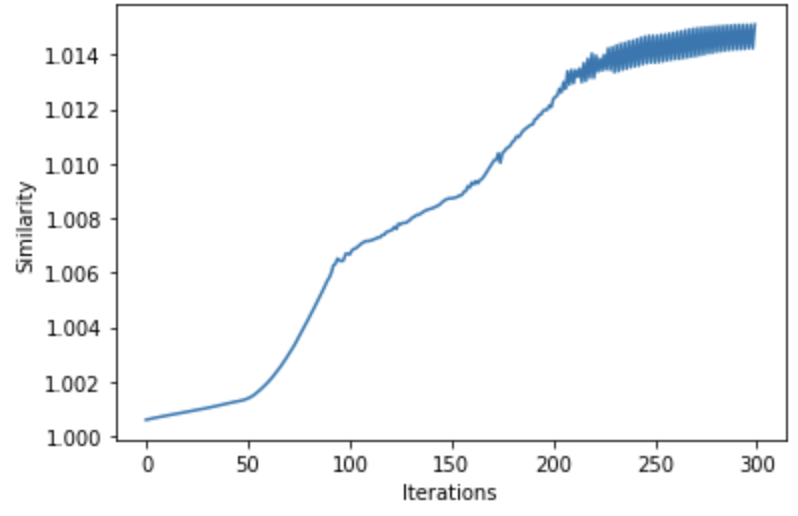
\includegraphics[width=0.4\linewidth]{Materials/affineNMIABLoss}
	\caption{Similarity at each iteration for affine registration between image A and B using NMI.}
	\label{affineNMIABLoss}
\end{figure}
We here note it is attempted to align the foreground of the images, however looking at \autoref{affineNMIABLoss} we see some volatile oscillation towards the end indicating we are using too big learning rates. This is likely the reason the the transformation matrix is not returning to 0 displacement. However, we see the houses and the car overlap slightly more than before. 
\subsection{Conclusion}
In conclusion we have seen SIFT and SURF detects roughly the same amount of features where ORB detects considerable less features. All three image descriptors perform somewhat bad when it comes to mean localization error, but this is likely due to aliasing or approximation error when transforming the images. When it comes to nearest neighbour mean average precision we see SIFT and ORB performs similar and fairly well, however SURF performs quite bad. This might be due to SIFT and ORB being both scale and rotation invariant, whereas SURF is only scale invariant. Lastly we have seen SIFT performs a lot better than both SURF and ORB when it comes to homography estimations, which is likely because SIFT both detects a lot of features and describes them well.\\
If we are to determine which of the three is better, it would depend on the task at hand. Although it is clear SIFT performs the best in the these experiments, it is also the slowest of the three. If the task requires fast feature matching it would not be possible to use SIFT, and we would need to trade performance for speed.